\documentclass[11pt,oneside]{article}	%use"amsart"insteadof"article"forAMSLaTeXformat
\usepackage{geometry}		%Seegeometry.pdftolearnthelayoutoptions.Therearelots.
\geometry{letterpaper}		%...ora4paperora5paperor...
%\geometry{landscape}		%Activateforforrotatedpagegeometry
%\usepackage[parfill]{parskip}		%Activatetobeginparagraphswithanemptylineratherthananindent
\usepackage{graphicx}				%Usepdf,png,jpg,orepsßwithpdflatex;useepsinDVImode
								%TeXwillautomaticallyconverteps-->pdfinpdflatex		
\usepackage{amssymb}
\usepackage[colorlinks]{hyperref}

%----macros begin---------------------------------------------------------------
\usepackage{color}
\usepackage{amsthm}

\def\conv{\mbox{\textrm{conv}\,}}
\def\aff{\mbox{\textrm{aff}\,}}
\def\E{\mathbb{E}}
\def\R{\mathbb{R}}
\def\Z{\mathbb{Z}}
\def\tex{\TeX}
\def\latex{\LaTeX}
\def\v#1{{\bf #1}}
\def\p#1{{\bf #1}}
\def\T#1{{\bf #1}}

\def\vet#1{{\left(\begin{array}{cccccccccccccccccccc}#1\end{array}\right)}}
\def\mat#1{{\left(\begin{array}{cccccccccccccccccccc}#1\end{array}\right)}}

\def\lin{\mbox{\rm lin}\,}
\def\aff{\mbox{\rm aff}\,}
\def\pos{\mbox{\rm pos}\,}
\def\cone{\mbox{\rm cone}\,}
\def\conv{\mbox{\rm conv}\,}
\newcommand{\homog}[0]{\mbox{\rm homog}\,}
\newcommand{\relint}[0]{\mbox{\rm relint}\,}

%----macros end-----------------------------------------------------------------

\title{Boolean Chains: set operations with topological chains
\footnote{This document is part of the \emph{Linear Algebraic Representation with CoChains} (LAR-CC) framework~\cite{cclar-proj:2013:00}. \today}
}
\author{TheAuthor}
%\date{}							%Activatetodisplayagivendateornodate

\begin{document}
\maketitle
%\nonstopmode

%----macros end-----------------------------------------------------------------
%>>>>>>>>>>>>>>>>>>>>>>>>>>>>>>>>>>>>>>>>>>>>>>>>>>>>>>>>>>>>>>>>>>>>>>>>>>>>>>>
\begin{abstract}
Boolean operations are a major addition to every geometric package. Union, intersection, difference and complementation of decomposed spaces are discussed and implemented in this module by making use of the Linear Algebraic Representation (LAR) introduced in~\cite{Dicarlo:2014:TNL:2543138.2543294}. First, the two finite decompositions are merged, by merging their vertices (0-cells of support spaces); then a Delaunay complex of set union of their boundary vertices is computed, and the shared $d$-chain is extracted and split, according to the cellular structure of the input $d$-chains. The results of a Boolean operation are finally computed by sum, product or difference of the (binary) coordinate representation of the (split) argument chains, by using the novel chain-basis resulted from such boundary-based splitting. Differently from the totality of algorithms known to the author, neither search nor traversal of some (complicated) data structure is performed by this algorithm. 
\end{abstract}

\tableofcontents
%<<<<<<<<<<<<<<<<<<<<<<<<<<<<<<<<<<<<<<<<<<<<<<<<<<<<<<<<<<<<<<<<<<<<<<<<<<<<<<<
\section{Introduction}
%>>>>>>>>>>>>>>>>>>>>>>>>>>>>>>>>>>>>>>>>>>>>>>>>>>>>>>>>>>>>>>>>>>>>>>>>>>>>>>>

In this section we introduce and shortly outline our novel algorithm for Boolean operations with chain of cells from different space decompositions implemented in this LAR-CC software module.

The input objects are denoted in the remainder as $X_1$ and $X_2$, and their finite cell decompositions as $\Lambda^1$ and $\Lambda^1$. Our goal is to compute $X = X_1\, op\, X_2$, where $op \in \{\cup ,\cap , - ,\ominus \}$ or $\complement X$, based on a common decomposition $\Lambda = \Lambda^1\, op\, \Lambda^2$, with $\Lambda$ being a suitably fragmented decomposition of the X space.

Of course, we aim to compute a minimal (in some sense) decomposition, making the best use of the LAR framework, based on CSR representation of sparse binary matrices and standard matrix algebra operations.
However, in this first implementation of the chain approach to Boolean operations, we are satisfied with a solution using simplicial triangulations of input spaces. Future revisions of our algorithm will be based on more general cellular complexes.

\subsection{User interface}

The API will contain the high-level binary functions \texttt{union}, \texttt{intersection}, \texttt{difference}, and \texttt{xor}. Each of them will call the same function \texttt{boolOps} and then suitably operates the two returned bit arrays, i.e.~the coordinate representations of the input spaces in the merged cell decomposition. The input parameters \texttt{lar1} and  \texttt{lar2} stand for two LAR models, each one constituted by a pair \texttt{(V,CV)}, i.e.~by the matrix \texttt{V} of vertex coordinates and by an integer array \texttt{CV} giving the vertex indices of each $d$-cell.

%-------------------------------------------------------------------------------
@D High-level Boolean operations
@{""" High level Boolean Application Programming Interface """
def larUnion(lar1,lar2): lar = boolOps(lar1,lar2); pass
def larIntersection(lar1,lar2): lar = boolOps(lar1,lar2); pass
def larDifference(lar1,lar2): lar = boolOps(lar1,lar2); pass
def larXor(lar1,lar2): lar = boolOps(lar1,lar2); pass
@}
%-------------------------------------------------------------------------------


%>>>>>>>>>>>>>>>>>>>>>>>>>>>>>>>>>>>>>>>>>>>>>>>>>>>>>>>>>>>>>>>>>>>>>>>>>>>>>>>
\section{Algorithm preview}
%>>>>>>>>>>>>>>>>>>>>>>>>>>>>>>>>>>>>>>>>>>>>>>>>>>>>>>>>>>>>>>>>>>>>>>>>>>>>>>>

The novel Boolean algorithm based on chains is summarised in this section. We will refer to the Boolean union; the other operators (intersection, difference, xor), will be derived accordingly.

\paragraph{Reordering of vertex coordinates}
First we embed both the (two) arguments $X_1, X_2$ in the same space, and order the vertex indices in three consecutive subsets, allocating in the first subset $V_1$ the vertices of $\Lambda^1$, in the second $V_{12}$ the (coincident or very-close) common vertices in $\Lambda^1\cap\Lambda^2$ , and the the third subset $V_2$ the remaining vertices of $\Lambda^2$. 

\paragraph{Input boundaries extraction}
Then we construct the boundary operators $\partial_d^1$ and $\partial_d^2$ over $\Lambda^1$ and $\Lambda^2$, respectively.
Then the boundary $(d-1)$-chains $B_{d-1}^1,B_{d-1}^2$ and $0$-chains $B_{0}^1,B_{0}^2$ are extracted, as relative to $V = V_{1} + V_{12} + V_{2} = V_{1} \cup V_{2} - V_{1} \cap V_{2}$.

\paragraph{Delaunay triangulation of boundary vertices}
The Delaunay triangulation $T$, with $|T| = \conv (X_1 \cup X_2)$, is then built over the 0-chain of boundary points $B = (B_{0}^1 \cup B_{0}^2) \subset V$.

\paragraph{Common simplices extraction}
The chain of $d$-simplices $T_d$ is finally classified in three subsets of cells, depending on the membership of their vertices:
\begin{enumerate}
\item the cells $T_d^1$ with only vertices in $V_{1} + V_{12}$, such that $|T_d^1|\subset X_1$;
\item the cells $T_d^2$ with only vertices in $V_{12} + V_{2}$, such that $|T_d^2|\subset X_2$;
\item the cells $T_d^{12}$ with vertices in both $V_{1}+V_{12}$ and $V_{12}+V_{2}$.
\end{enumerate}

\paragraph{Common simplices classification}
Both $T_d^1$ and $T_d^2$ can be excluded from any further consideration. Conversely, the $d$-simplices in $T_d^{12}$ can be in turn classified in three disjoint subsets: 
\begin{enumerate}
\item $T_{{in}}\subset T_d^{12}$: those internal to both the boundaries;
\item $T_{{out}}\subset T_d^{12}$: those external to both the boundaries;
\item $T_{{on}}\subset T_d^{12}$: those external to one boundary and internal to the other.
\end{enumerate}

\paragraph{Pivot simplices splitting}
Both $T_{{in}}$ and $T_{{out}}$ can be excluded from any further consideration. The cells in $T_{{on}}$ will be used to refine both $B_{d-1}^1,B_{d-1}^2$ and their coboundaries, so that the result of the target Boolean operation can be finally constructed. 


%-------------------------------------------------------------------------------
\subsection{The top-level algorithm}
%-------------------------------------------------------------------------------
@D Boolean subdivided complex
@{@< Place the vertices of Boolean arguments in a common space @>
def boolOps(lar1,lar2,cell='simplex', facets1=None,facets2=None):
	(V1,CV1),(V2,CV2) = lar1,lar2
	n1,n2 = len(V1),len(V2)
	V, CV1, CV2, n12 = vertexSieve(lar1, lar2)
	CV = Delaunay(array(V)).vertices
	BV1, BV2 = boundaryVertices( V, CV1,CV2, cell, facets1,facets2 )
	print "\n BV1 =",BV1
	print "\n BV2 =",BV2
	@< Delaunay triangulation of boundary vertices @>
	@< Common simplices extraction @>
	return V,n1,n2,n12, BV1, BV2
@}
%-------------------------------------------------------------------------------



%>>>>>>>>>>>>>>>>>>>>>>>>>>>>>>>>>>>>>>>>>>>>>>>>>>>>>>>>>>>>>>>>>>>>>>>>>>>>>>>
\section{Boolean algorithm}
%>>>>>>>>>>>>>>>>>>>>>>>>>>>>>>>>>>>>>>>>>>>>>>>>>>>>>>>>>>>>>>>>>>>>>>>>>>>>>>>
%-------------------------------------------------------------------------------
\subsection{Reordering of vertex coordinates}
%-------------------------------------------------------------------------------
A global reordering of vertex coordinates is executed as the first step of the Boolean algorithm, in order to eliminate the duplicate vertices, by substituting duplicate vertex copies (coming from two close points) with a single instance. 

Two dictionaries are created, then merged in a single dictionary, and finally split into three subsets of (vertex,index) pairs, with the aim of rebuilding the input representations, by making use of a novel and more useful vertex indexing.

The union set of vertices is finally reordered using the three subsets of vertices belonging (a) only to the first argument, (b) only to the second argument and (c) to both, respectively denoted as $V_1, V_2, V_{12}$. A top-down description of this initial computational step is provided by the set of macros discussed in this section.

%-------------------------------------------------------------------------------
@D Place the vertices of Boolean arguments in a common space
@{""" First step of Boolean Algorithm """
@< Initial indexing of vertex positions @>
@< Merge two dictionaries with keys the point locations @>
@< Filter the common dictionary into three subsets @>
@< Compute an inverted index to reorder the vertices of Boolean arguments @>
@< Return the single reordered pointset and the two $d$-cell arrays @>
@}
%-------------------------------------------------------------------------------

%-------------------------------------------------------------------------------
\subsubsection{Re-indexing of vertices}
%-------------------------------------------------------------------------------

\paragraph{Initial indexing of vertex positions}
The input LAR models are located in a common space by (implicitly) joining \texttt{V1} and \texttt{V2} in a same array, and (explicitly) shifting the vertex indices in \texttt{CV2} by the length of \texttt{V1}.
%-------------------------------------------------------------------------------
@D Initial indexing of vertex positions
@{from collections import defaultdict, OrderedDict

""" TODO: change defaultdict to OrderedDefaultdict """

class OrderedDefaultdict(collections.OrderedDict):
    def __init__(self, *args, **kwargs):
        if not args:
            self.default_factory = None
        else:
            if not (args[0] is None or callable(args[0])):
                raise TypeError('first argument must be callable or None')
            self.default_factory = args[0]
            args = args[1:]
        super(OrderedDefaultdict, self).__init__(*args, **kwargs)

    def __missing__ (self, key):
        if self.default_factory is None:
            raise KeyError(key)
        self[key] = default = self.default_factory()
        return default

    def __reduce__(self):  # optional, for pickle support
        args = (self.default_factory,) if self.default_factory else tuple()
        return self.__class__, args, None, None, self.iteritems()


def vertexSieve(model1, model2):
	from lar2psm import larModelBreak
	V1,CV1 = larModelBreak(model1) 
	V2,CV2 = larModelBreak(model2)
	n = len(V1); m = len(V2)
	def shift(CV, n): 
		return [[v+n for v in cell] for cell in CV]
	CV2 = shift(CV2,n)
@}
%-------------------------------------------------------------------------------

\paragraph{Merge two dictionaries with point location as keys}
Since currently \texttt{CV1} and \texttt{CV2} point to a set of vertices larger than their initial sets 
\texttt{V1} and \texttt{V2}, we index the set $\texttt{V1} \cup \texttt{V2}$ using a Python \texttt{defaultdict} dictionary, in order to avoid errors of "missing key". As dictionary keys, we use the string representation of the vertex position vector provided by the \texttt{vcode} function given in the Appendix.
%-------------------------------------------------------------------------------
@D Merge two dictionaries with keys the point locations
@{	vdict1 = defaultdict(list)
	for k,v in enumerate(V1): vdict1[vcode(v)].append(k) 
	vdict2 = defaultdict(list)
	for k,v in enumerate(V2): vdict2[vcode(v)].append(k+n) 
	
	vertdict = defaultdict(list)
	for point in vdict1.keys(): vertdict[point] += vdict1[point]
	for point in vdict2.keys(): vertdict[point] += vdict2[point]
@}
%-------------------------------------------------------------------------------

\paragraph{Example of string coding of a vertex position}
The position vector of a point of real coordinates is provided by the function \texttt{vcode}.
An example of coding is given below. The \emph{precision} of the string representation can be tuned at will.
{\small
\begin{verbatim}
>>> vcode([-0.011660381062724849, 0.297350056848685860])
'[-0.0116604, 0.2973501]'
\end{verbatim}}



\paragraph{Filter the common dictionary into three subsets}
\texttt{Vertdict}, dictionary of vertices, uses as key the position vectors of vertices coded as string, and as values the list of integer indices of vertices on the given position. If the point position belongs either to the first or to second argument only, it is stored in \texttt{case1} or \texttt{case2} lists respectively. If the position (\texttt{item.key}) is shared between two vertices, it is stored in \texttt{case12}.
The variables \texttt{n1}, \texttt{n2}, and \texttt{n12} remember the number of vertices respectively stored in each repository.
%-------------------------------------------------------------------------------
@D Filter the common dictionary into three subsets
@{	case1, case12, case2 = [],[],[]
	for item in vertdict.items():
		key,val = item
		if len(val)==2:  case12 += [item]
		elif val[0] < n: case1 += [item]
		else: case2 += [item]
	n1 = len(case1); n2 = len(case12); n3 = len(case2)
@}
%-------------------------------------------------------------------------------

\paragraph{Compute an inverted index to reorder the vertices of Boolean arguments}
The new indices of vertices are computed according with their position within the storage repositories \texttt{case1}, \texttt{case2}, and \texttt{case12}. Notice that every \texttt{item[1]} stored in \texttt{case1} or \texttt{case2} is a list with only one integer member. Two such values are conversely stored in each \texttt{item[1]} within \texttt{case12}.
%-------------------------------------------------------------------------------
@D Compute an inverted index to reorder the vertices of Boolean arguments 
@{
	invertedindex = list(0 for k in range(n+m))
	for k,item in enumerate(case1):
		invertedindex[item[1][0]] = k
	for k,item in enumerate(case12):
		invertedindex[item[1][0]] = k+n1
		invertedindex[item[1][1]] = k+n1
	for k,item in enumerate(case2):
		invertedindex[item[1][0]] = k+n1+n2
@}
%-------------------------------------------------------------------------------

%-------------------------------------------------------------------------------
\subsubsection{Re-indexing of d-cells}
%-------------------------------------------------------------------------------

\paragraph{Return the single reordered pointset and the two $d$-cell arrays}
We are now finally ready to return two reordered LAR models defined over the same set \texttt{V} of vertices, and where (a) the vertex array \texttt{V} can be written as the union of three disjoint sets of points $C_1,C_{12},C_2$; (b) the $d$-cell array \texttt{CV1} is indexed over $C_1\cup C_{12}$; (b) the $d$-cell array \texttt{CV2} is indexed over $C_{12}\cup C_{2}$. 

The \texttt{vertexSieve} function will return the new reordered vertex set $V = (V_1 \cup V_2) \setminus (V_1 \cap V_2)$, the two renumbered $s$-cell sets \texttt{CV1} and \texttt{CV2}, and the size \texttt{len(case12)} of $V_1 \cap V_2$.
%-------------------------------------------------------------------------------
@D Return the single reordered pointset and the two $d$-cell arrays
@{
	V = [eval(p[0]) for p in case1] + [eval(p[0]) for p in case12] + [eval(
				p[0]) for p in case2]
	CV1 = [sorted([invertedindex[v] for v in cell]) for cell in CV1]
	CV2 = [sorted([invertedindex[v] for v in cell]) for cell in CV2]
	return V, CV1, CV2, len(case12)
@}
%-------------------------------------------------------------------------------


\subsubsection{Example of input with some coincident vertices}
In this example we give two very simple LAR representations of 2D cell complexes, with some coincident vertices, and go ahead to re-index the vertices, according to the method implemented by the function \texttt{vertexSieve}.

%-------------------------------------------------------------------------------
@o test/py/boolean/test02.py
@{@< Initial import of modules @>
from boolean import *
V1 = [[1,1],[3,3],[3,1],[2,3],[2,1],[1,3]]
V2 = [[1,1],[1,3],[2,3],[2,2],[3,2],[0,1],[0,0],[2,0],[3,0]]
CV1 = [[0,3,4,5],[1,2,3,4]]
CV2 = [[3,4,7,8],[0,1,2,3,5,6,7]]
model1 = V1,CV1; model2 = V2,CV2
VIEW(STRUCT([ 
	COLOR(CYAN)(SKEL_1(STRUCT(MKPOLS(model1)))), 
	COLOR(RED)(SKEL_1(STRUCT(MKPOLS(model2)))) ]))
V, n1,n2,n12,BV1,BV2 = boolOps(model1,model2)
# VIEW(SKEL_1(STRUCT(MKPOLS((V, CV_un[:n1]+CV_int )))))
# VIEW(SKEL_1(STRUCT(MKPOLS((V, CV_un[n1-n12:]+CV_int )))))
@}
%-------------------------------------------------------------------------------

\paragraph{Example discussion} 
The aim of the \texttt{vertexSieve} function is twofold: (a) eliminate vertex duplicates before entering the main part of the Boolean algorithm; (b) reorder the input representations so that it becomes less expensive to check whether a 0-cell can be shared by both the arguments of a Boolean expression, so that its coboundaries must be eventually split. Remind that for any set it is:
\[
|A\cup B| = |A|+|B|-|A\cap B|.
\]
Let us notice that in the previous example
\[
|V| = |V_1 \cup V_2| = 12 \leq |V_1|+|V_2| = 6+9 = 15,
\]
and that 
\[
|V_1|+|V_2| - |V_1 \cup V_2| = 15 - 12 = 3 = |C_{12}| = |V_1 \cap V_2|,
\]
where $C_{12}$ is the subset of vertices with duplicated instances.
%-------------------------------------------------------------------------------
@D Output from \texttt{test/py/boolean/test02.py}
@{V   = [[3.0,1.0],[2.0,1.0],[3.0,3.0],[1.0,1.0],[1.0,3.0],[2.0,3.0],
		 [3.0,2.0],[2.0,0.0],[2.0,2.0],[0.0,0.0],[3.0,0.0],[0.0,1.0]]
CV1 = [[3,5,1,4],[2,0,5,1]]
CV2 = [[8,6,7,10],[3,4,5,8,11,9,7]]
@}
%-------------------------------------------------------------------------------
Notice also that \texttt{V} has been reordered in three consecutive subsets $C_{1},C_{12},C_{2}$ such that \texttt{CV1} is indexed within $C_{1}\cup C_{12}$, whereas \texttt{CV2} is indexed within $C_{12}\cup C_{2}$. In our example we have  $C_{12}=\{\texttt{3,4,5}\}$: 
%-------------------------------------------------------------------------------
@D Reordering of vertex indexing of cells
@{
>>> sorted(CAT(CV1))
[0, 1, 1, 2, 3, 4, 5, 5]
>>> sorted(CAT(CV2))
[3, 4, 5, 6, 7, 7, 8, 8, 9, 10, 11]
@}
%-------------------------------------------------------------------------------
\paragraph{Cost analysis} 
Of course, this reordering after elimination of duplicate vertices will allow to perform a cheap $O(n)$ discovering of (Delaunay) cells whose vertices belong both to \texttt{V1} \emph{and} to \texttt{V2}. 
Actually, the \emph{same test} can be now used both when the vertices of the input arguments are all different, \emph{and} when they have some coincident vertices.
The total cost of such pre-processing, executed using dictionaries, is $O(n\ln n)$.

%-------------------------------------------------------------------------------
\subsection{Input boundaries extraction}
%-------------------------------------------------------------------------------

The matrix of the boundary operators of the boolean arguments $\Lambda_1$ and $\Lambda_2$ are computed here as supported by the novel vertex set $V := V_1 \cup V_2$. Both the characteristic matrices $M_d$ and $M_{d-1}$ are needed to compute a $[\partial_d]$ matrix (see Reference~\cite{Dicarlo:2014:TNL:2543138.2543294}). Hence we start this section by computing the new basis of $(d-1)$-faces $\texttt{FV} := \texttt{CSR}(M_{d-1})$, and then compute the two subsets $B_1,B_2 \subset V$ of boundary vertices (upon the joint Delaunay complex \texttt{V}), where
\[
B_1 = [\mathcal{VF}^1]\, [\partial_d^1]\,\mathbf{1},
\quad\mbox{and}\quad
B_2 = [\mathcal{VF}^2]\, [\partial_d^2]\,\mathbf{1}.
\]
where $[\mathcal{VF}^1]^\top = \texttt{CSR(FV1)}$ and $[\mathcal{VF}^2]^\top = \texttt{CSR(FV2)}$,
and where \texttt{FV1} and \texttt{FV2} are the relations \emph{face-vertices} computed from the relation \texttt{CV} supported by the \emph{joint} Delaunay vertex set. 

\paragraph{Compute the boundary vertices of both arguments}
The two bases of $d$-cells, given as input to the \texttt{boundaryVertices} function below, were already renumbered. In other words, their vertices currently belong to the common Delaunay complex. Therefore, the subsequent calls to \texttt{larSimplexFacets} also return two sets of boundary facets, denoted as \texttt{BF1} and \texttt{BF2}, are supported by the Delaunay complex. \texttt{BV1} and \texttt{BV2} contain the boundary vertex indices of the input cells \texttt{CV1} and \texttt{CV2}.

%-------------------------------------------------------------------------------
@D Compute boundary vertices of both arguments
@{""" Second stage of Boolean operations """
def boundaryVertices( V, CV1,CV2, cell='simplex', facets1=None,facets2=None ):
	if cell=='simplex': 
		FV1 = larSimplexFacets(CV1)
		FV2 = larSimplexFacets(CV2)
	elif cell=='cuboid': 
		FV1 = facets1
		print "\n FV1 =",FV1
		FV2 = facets2
		print "\n FV2 =",FV2
	BF1 = boundaryCells(CV1,FV1)
	print "\n BF1 =",BF1
	BF2 = boundaryCells(CV2,FV2)
	BV1 = list(set(CAT([ FV1[f] for f in BF1 ])))
	BV2 = list(set(CAT([ FV2[f] for f in BF2 ])))
	VIEW(STRUCT([ 
		COLOR(GREEN)(STRUCT(AA(MK)([V[v] for v in BV1]))), 
		COLOR(YELLOW)(STRUCT(AA(MK)([V[v] for v in BV2]))) ]))
	return BV1, BV2
@}
%-------------------------------------------------------------------------------
%-------------------------------------------------------------------------------
\subsection{Delaunay triangulation of boundary vertices}
%-------------------------------------------------------------------------------

The Delaunay complex is computed on the on the 0-chain of boundary vertices $B\subset V$, using some efficient package for dimensional-independent Delaunay computation. In the following  we will utilize the \texttt{scipy.spatial.Delaunay} sub-package, that can be used with both 2D and 3D points. 

%-------------------------------------------------------------------------------
@D Delaunay triangulation of boundary vertices
@{""" Delaunay triangulation of boundary vertices """
B = [V[v] for v in BV1+BV2]
CV = Delaunay(array(B)).vertices
VIEW(STRUCT([
	EXPLODE(1.2,1.2,1.2)(MKPOLS((B,CV))),
	COLOR(CYAN)(SKEL_1(EXPLODE(1.2,1.2,1.2)(MKPOLS((V,CV1))))),
	COLOR(MAGENTA)(SKEL_1(EXPLODE(1.2,1.2,1.2)(MKPOLS((V,CV2)))))
]))
""" back-indicize globally (original common vertices) """
BV = [v for k,v in enumerate(BV1+BV2)]
CV = [[BV[v] for v in cell] for cell in CV]
@}
%-------------------------------------------------------------------------------

\begin{figure}[htbp] %  figure placement: here, top, bottom, or page
   \centering
   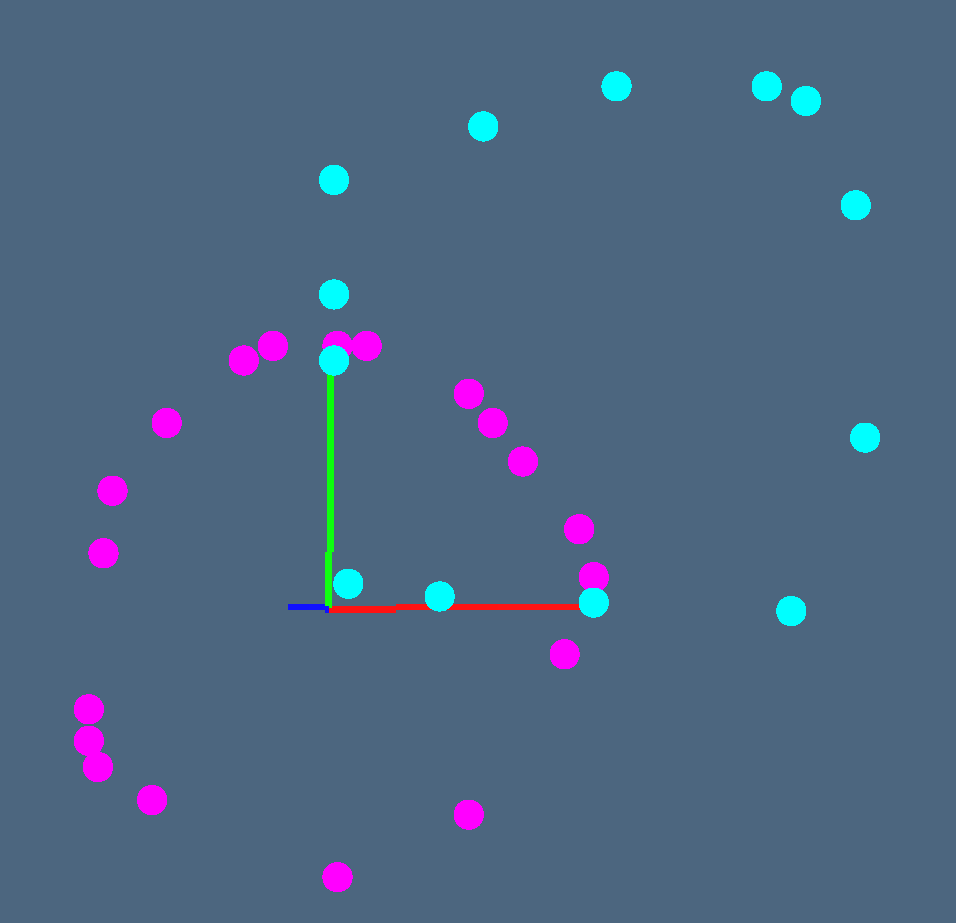
\includegraphics[height=0.24\textwidth,width=0.24\textwidth]{images/chains1} 
   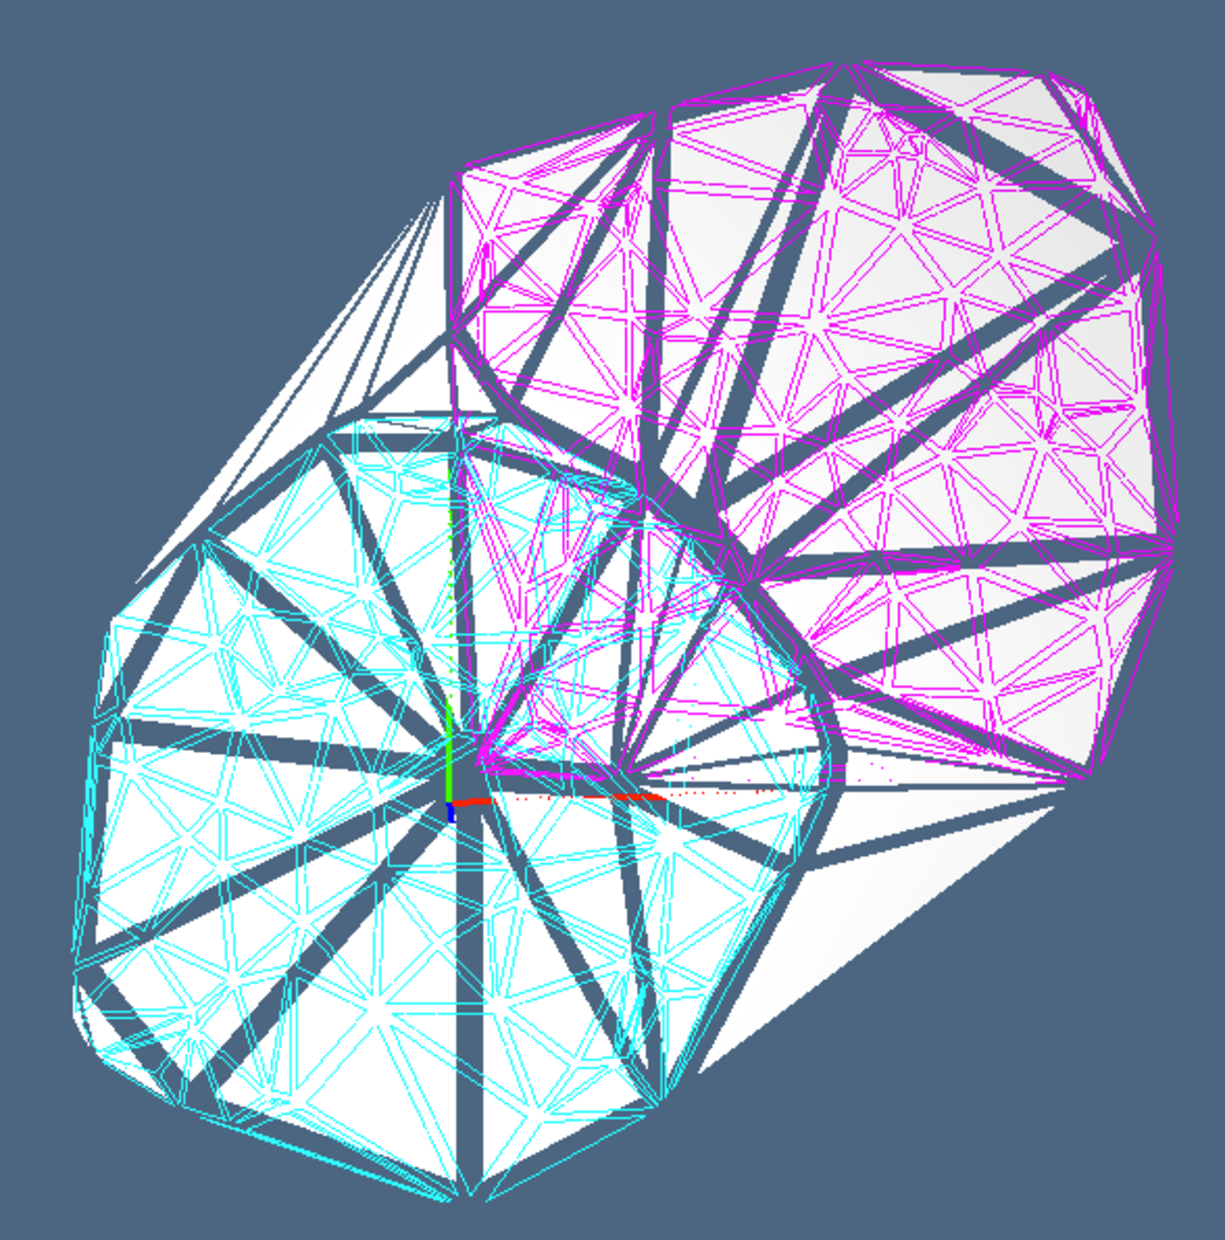
\includegraphics[height=0.24\textwidth,width=0.24\textwidth]{images/chains2} 
   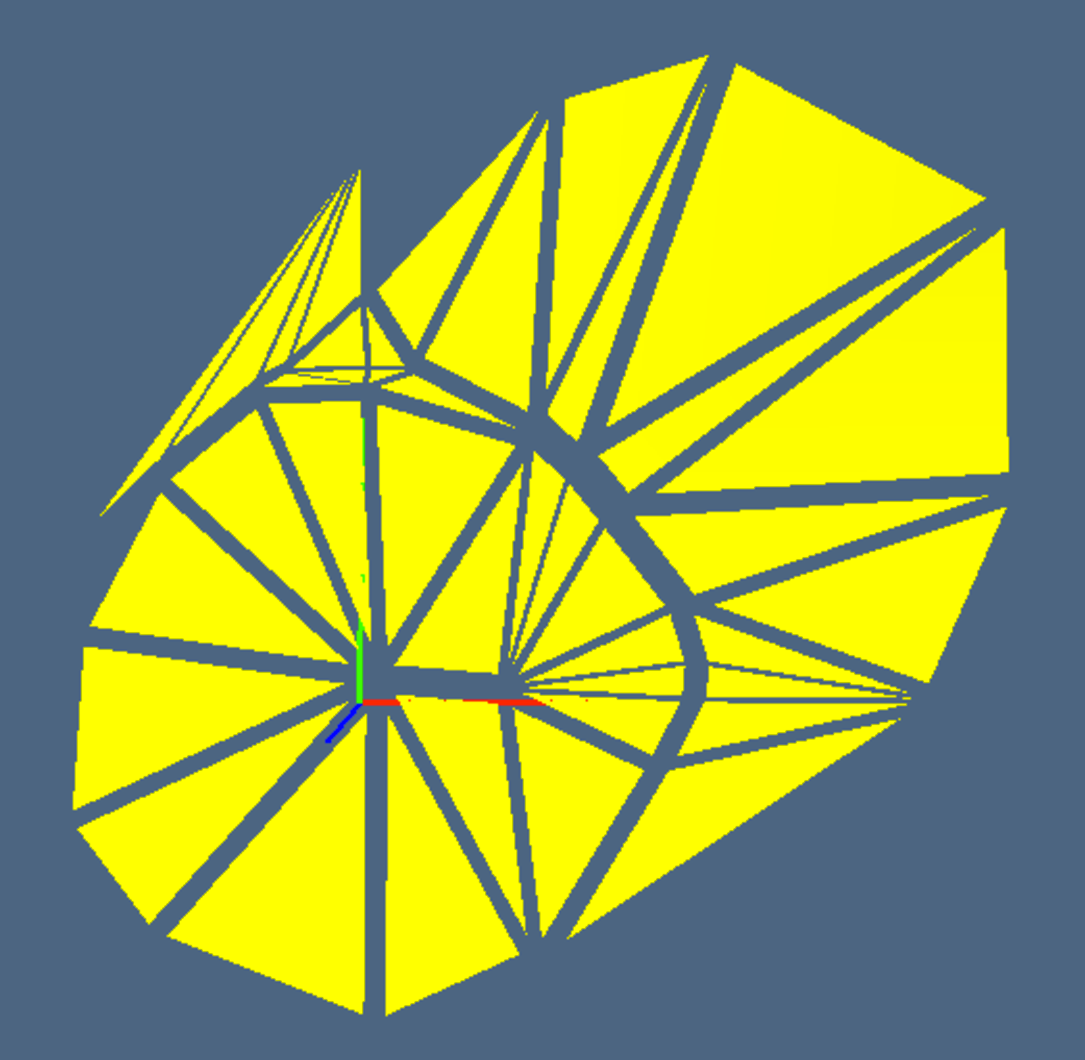
\includegraphics[height=0.24\textwidth,width=0.24\textwidth]{images/chains3} 
   
\includegraphics[height=0.24\textwidth,width=0.24\textwidth]{images/chains4} 
   \caption{(a) 0-chains of boundary vertices; (b) Delaunay triangulation; (c) chain of $d$-cells with mixed vertices; (d) classification into 4 chains: out.A.out.B (white), out.A.in.B (cyan), in.A.out.B (magenta), in.A.in.B (yellow),}
   \label{fig:example}
\end{figure}

%-------------------------------------------------------------------------------
\subsection{Common simplices extraction}
%-------------------------------------------------------------------------------


%-------------------------------------------------------------------------------
@D Common simplices extraction
@{""" Common simplices extraction """
CV_un, CV_int = splitDelaunayComplex(CV,n1,n2,n12)
print "\n CV_un =",CV_un
print "\n CV_int =",CV_int
VIEW(COLOR(YELLOW)(EXPLODE(1.2,1.2,1)(MKPOLS((V,CV_int)))))
@}
%-------------------------------------------------------------------------------


\paragraph{Partition of the joint Delaunay complex} 

The \texttt{splitDelaunayComplex} function is used to partition the Delaunay complex $\Sigma\equiv\texttt{CV}$, previously computed on $V_1 \cup V_2$, into two subcomplexes $\Sigma_\sqcup$ and $\Sigma_\cap$, respectively characterised by the fact that the cells  are either supported by (i.e.~are convex combination of)  $d+1$ vertices belonging to the same argument, or by vertices in both arguments.
The two sets of cells returned by the function are respectively denoted \texttt{cells\_union} and \texttt{cells\_intersection}. They are computed efficiently in time $O(n)$ by using the previous reordering of vertices, i.e.~the vertex partition in three disjoint subsets delimited by four ordered integer indices $k_0 < k_1 \leq k_2 < k_3$:
\[
V_1 \cup V_2 = 
\{v_k\ |\ k_0\leq k< k_1\} \cup
\{v_k\ |\ k_1\leq k< k_2\} \cup
\{v_k\ |\ k_2\leq k< k_3\}
\]
where
\[
k_0 =0, \quad k_1 =n_1-n_{12}, \quad k_2 =n_1, \quad  k_3=n_1+n_2-n_{12},
\]
with $n_1=|V_1|$, $n_2=|V_2|$, $n_1, n_2\not=0$, and $n_{12}=|V_1\cap V_2|$.

%-------------------------------------------------------------------------------
@d Partition of the Delaunay complex in two sub complexes
@{def splitDelaunayComplex(CV,n1,n2,n12):
	def test(cell):
		return any([v<n1 for v in cell]) and any([v>=(n1-n12) for v in cell])
	cells_intersection, cells_union = [],[]
	for cell in CV: 
		if test(cell): cells_intersection.append(cell)
		else: cells_union.append(cell)
	return cells_union,cells_intersection
@}
%-------------------------------------------------------------------------------




%-------------------------------------------------------------------------------
\subsection{Common simplices classification}
%-------------------------------------------------------------------------------
%-------------------------------------------------------------------------------
\subsection{Pivot simplices splitting}
%-------------------------------------------------------------------------------
%>>>>>>>>>>>>>>>>>>>>>>>>>>>>>>>>>>>>>>>>>>>>>>>>>>>>>>>>>>>>>>>>>>>>>>>>>>>>>>>
\section{Exporting the boolean module}
%<<<<<<<<<<<<<<<<<<<<<<<<<<<<<<<<<<<<<<<<<<<<<<<<<<<<<<<<<<<<<<<<<<<<<<<<<<<<<<<

The \texttt{boolean.py} module is exported to the library \texttt{lar-cc/lib}. Therefore many of the macros developed in this module are expanded and written to an external file.

%------------------------------------------------------------------
@o lib/py/boolean.py
@{""" Module with Boolean operators using chains and CSR matrices """
@< Initial import of modules @>
@< Symbolic utility to represent points as strings @>
@< High-level Boolean operations @>
@< Boolean subdivided complex @>
@< Compute boundary vertices of both arguments @>
@< Partition of the Delaunay complex in two sub complexes @>
@< Random data input @>
@< Visualization of subsets of cells @>
@}
%------------------------------------------------------------------

\subsection{Visualization of the Boolean algorithm}

\paragraph{Display of colored cell numbers}

%------------------------------------------------------------------
@D Visualization of subsets of cells
@{def cellNames(model,cells, color=BLACK):
	V,CV= model
	print "\n CV =",CV
	print "\n cells =",cells
	texts = []
	for k,cell in enumerate(cells):
		centroid = CCOMB([V[v] for v in cell])
		print "centroid =",centroid
		d = len(centroid)
		texts += [ T(range(1,d+1))(centroid)(S(range(1,d+1))([0.02 
						for h in range(d)])(TEXTWITHATTRIBUTES()(str(k)))) ]
	return AA(COLOR(color))(texts)
@}
%------------------------------------------------------------------

%>>>>>>>>>>>>>>>>>>>>>>>>>>>>>>>>>>>>>>>>>>>>>>>>>>>>>>>>>>>>>>>>>>>>>>>>>>>>>>>
\section{Examples}
%>>>>>>>>>>>>>>>>>>>>>>>>>>>>>>>>>>>>>>>>>>>>>>>>>>>>>>>>>>>>>>>>>>>>>>>>>>>>>>>
%-------------------------------------------------------------------------------
\subsection{Generation of random data}
%-------------------------------------------------------------------------------
%-------------------------------------------------------------------------------

We found useful to drive the development of new modules using randomly generated data, so that every upcoming execution of the developed algorithms is naturally driven to be challenged by different data.

\subsubsection{Testing the main algorithm}

\paragraph{Write the test executable file}




\subsubsection{Lowest-level space generation procedures}

\paragraph{Random data input} 

%------------------------------------------------------------------
@D Random data input 
@{@< Generation of $n$ random points in the unit $d$-disk @>
@< Generation of $n$ random points in the standard $d$-cuboid @>
@< Triangulation of random points @>
@}
%------------------------------------------------------------------

\paragraph{Random points in unit disk} 
First we generate a  set of $n$ random points in the unit $D^d$ disk centred on the origin, to be subsequently used to generate a random Delaunay complex of variable granularity.

%------------------------------------------------------------------
@D Generation of $n$ random points in the unit $d$-disk 
@{def randomPointsInUnitCircle(n=200,d=2, r=1):
	points = random.random((n,d)) * ([2*math.pi]+[1]*(d-1))
	return [[SQRT(p[1])*COS(p[0]),SQRT(p[1])*SIN(p[0])] for p in points]
	## TODO: correct for $d$-sphere

if __name__=="__main__":
	VIEW(STRUCT(AA(MK)(randomPointsInUnitCircle()))) 
@}
%------------------------------------------------------------------

\paragraph{Random points in the standard $d$-cuboid} 
A set of $n$ random $d$-points is then generated within the standard $d$-cuboid, i.e.~withing the $d$-dimensional interval with a vertex on the origin.

%------------------------------------------------------------------
@D Generation of $n$ random points in the standard $d$-cuboid 
@{def randomPointsInUnitCuboid(n=200,d=2):
	return random.random((n,d)).tolist()

if __name__=="__main__":
	VIEW(STRUCT(AA(MK)(randomPointsInUnitCuboid()))) 
@}
%------------------------------------------------------------------



\paragraph{Triangulation of random points} The Delaunay triangulation of \texttt{randomPointsInUnitCircle} is generated by the following macro.


%------------------------------------------------------------------
@D Triangulation of random points
@{from scipy.spatial import Delaunay
def randomTriangulation(n=200,d=2,out='disk'):
	if out == 'disk':
		V = randomPointsInUnitCircle(n,d)
	elif out == 'cuboid':
		V = randomPointsInUnitCuboid(n,d)
	CV = Delaunay(array(V)).vertices
	model = V,CV
	return model

if __name__=="__main__":
	from lar2psm import *
	VIEW(EXPLODE(1.5,1.5,1)(MKPOLS(model)))
@}
%------------------------------------------------------------------
%-------------------------------------------------------------------------------
\subsection{Unit tests}
%-------------------------------------------------------------------------------

\subsubsection{First Boolean stage}

Some unit tests of the first Boolean stage are discussed in the following. They are mainly aimed to check a correct execution of the filtering of common vertices with renumbering of the union set of vertices, and to the consequential redefinition of the $d$-cell basis.

\paragraph{Union of 2D non-structured grids}

%------------------------------------------------------------------
@o test/py/boolean/test01.py
@{""" Union of 2D non-structured grids """
@< Initial import of modules @>
from boolean import *
from lar2psm import *
from myfont import *
model1 = randomTriangulation(100,2,'disk')
V1,CV1 = model1
VIEW(EXPLODE(1.5,1.5,1)(MKPOLS(model1)+cellNames(model1,CV1,MAGENTA)))
model2 = randomTriangulation(100,2,'cuboid')
V2,CV2 = model2
V2 = larScale( [2,2])(V2)
model2 = V2,CV2 
VIEW(EXPLODE(1.5,1.5,1)(MKPOLS(model2)+cellNames(model2,CV2,RED)))
V, n1,n2,n12,BV1,BV2 = boolOps(model1,model2)
@}
%------------------------------------------------------------------

\paragraph{Union of 3D non-structured grids}

%------------------------------------------------------------------
@o test/py/boolean/test05.py
@{""" Union of 3D non-structured grids """
@< Initial import of modules @>
from boolean import *
model1 = randomTriangulation(100,3,'cuboid')
V1,CV1 = model1
V1 = larScale( [2,2,2])(V1)
V1 = larTranslate( [-1,-1,-1])(V1)
model1 = V1,CV1 
VIEW(EXPLODE(1.5,1.5,1.5)(MKPOLS(model1)+cellNames(model1,CV1,MAGENTA)))
model2 = randomTriangulation(100,3,'cuboid')
V2,CV2 = model2
V2 = larScale( [2,2,2])(V2)
model2 = V2,CV2 
VIEW(EXPLODE(1.5,1.5,1.5)(MKPOLS(model2)+cellNames(model2,CV2,RED)))
V, n1,n2,n12;BV1,BV2 = boolOps(model1,model2)
@}
%------------------------------------------------------------------


\paragraph{Union of structured grids}

%------------------------------------------------------------------
@o test/py/boolean/test04.py
@{""" test program for the boolean module """
@< Initial import of modules @>
from boolean import *
blue = larSimplexGrid([30,60])
V2,CV2 = larSimplexGrid([70,40])
V2 = larTranslate( [.5,.5])(V2)
red = V2,CV2
VIEW(EXPLODE(1.5,1.5,1)(MKPOLS(blue) ))
VIEW(EXPLODE(1.5,1.5,1)(MKPOLS(red) ))
V, CV1, CV2, n12 = vertexSieve(red,blue)
V, n1,n2,n12 = boolOps(red,blue)
CV = Delaunay(array(V)).vertices
@}
%------------------------------------------------------------------


model = checkModel(larHollowCyl(0.8,1,1,angle=PI/4)([12,2,2]))
VIEW(STRUCT(MKPOLS(model)))
model = checkModel(larHollowSphere(0.8,1,PI/6,PI/4)([6,12,2]))


\paragraph{Union of structured grids}

%------------------------------------------------------------------
@o test/py/boolean/test06.py
@{""" test program for the boolean module """
@< Initial import of modules @>
from mapper import *
from boolean import boolOps
blue = larHollowCyl(0.8,1,1,angle=PI/4)([6,2,5])
VIEW(STRUCT(MKPOLS(blue)))
V1,FV1 = larHollowCylFacets(0.8,1,1,angle=PI/4)([6,2,5])
assert blue[0]==V1
print "*** len(V1) =",len(V1)
red = larHollowSphere(0.8,1,PI/6,PI/4)([6,12,2])
VIEW(STRUCT(MKPOLS(red)))
V2,FV2= larHollowSphereFacets(0.8,1,PI/6,PI/4)([6,12,2])
assert red[0]==V2
print "*** len(V2) =",len(V2)
V, n1,n2,n12,BV1,BV2 = boolOps(blue,red,'cuboid',FV1,FV2)
@}
%------------------------------------------------------------------

%-------------------------------------------------------------------------------
\subsection{Examples}
%-------------------------------------------------------------------------------
%>>>>>>>>>>>>>>>>>>>>>>>>>>>>>>>>>>>>>>>>>>>>>>>>>>>>>>>>>>>>>>>>>>>>>>>>>>>>>>>
\appendix
%>>>>>>>>>>>>>>>>>>>>>>>>>>>>>>>>>>>>>>>>>>>>>>>>>>>>>>>>>>>>>>>>>>>>>>>>>>>>>>>
%-------------------------------------------------------------------------------
\section{Utility functions}
%-------------------------------------------------------------------------------
@D Initial import of modules
@{from pyplasm import *
from scipy import *
import os,sys
""" import modules from larcc/lib """
sys.path.insert(0, 'lib/py/')
from lar2psm import *
from simplexn import *
from larcc import *
from largrid import *
from myfont import *
from mapper import *
@}
%------------------------------------------------------------------
\subsection{Numeric utilities}

A small set of utilityy functions is used to transform a point representation as array of coordinates into a string of fixed format to be used as point key into python dictionaries.

%------------------------------------------------------------------
@D Symbolic utility to represent points as strings
@{""" TODO: use package Decimal (http://docs.python.org/2/library/decimal.html) """
ROUND_ZERO = 1E-07
def round_or_zero (x,prec=7):
	"""
	Decision procedure to approximate a small number to zero.
	Return either the input number or zero.
	"""
	def myround(x):
		return eval(('%.'+str(prec)+'f') % round(x,prec))
	xx = myround(x)
	if abs(xx) < ROUND_ZERO: return 0.0
	else: return xx

def prepKey (args): return "["+", ".join(args)+"]"

def fixedPrec(value):
	if abs(value - int(value))<ROUND_ZERO: value = int(value)
	out = ('%0.7f'% value).rstrip('0')
	if out == '-0.': out = '0.'
	return out
	
def vcode (vect): 
	"""
	To generate a string representation of a number array.
	Used to generate the vertex keys in PointSet dictionary, and other similar operations.
	"""
	return prepKey(AA(fixedPrec)(vect))
@}
%------------------------------------------------------------------





\bibliographystyle{amsalpha}
\bibliography{boolean}

\end{document}
